\section{Theorie}
\label{sec:Theorie}

Grundsätzlich besitzt ein Hüllenelektron den Bahndrehimpuls $\vec{j}$ und den Eigendrehimpuls $\vec{s}$, auch Spin genannt. Die Ladung $e_0$ und die Masse $m_0$ des Elektrons stellt eine Verbindung zwischen den Drehimpulsen und dem magnetischem Moment her. Für das auf die Drehimpulseinheit $\hbar$ (m=0) bezogene magnetische Moment ergibt sich folgender Wert:
\begin{align}
	\mu_z=-\frac{1}{2}e_0\frac{\hbar}{m_0} =: \mu_B
\end{align}
Diese Wert wird auch als Bohrsches Magneton $\mu_B$ bezeichnet. Durch einsetzen in die obige Gleichung ergibt sich das magnetische Moment zum Bahndrehimpuls
\begin{align}
	\vec{\mu}_l=-\mu_B\frac{\vec{l}}{\hbar}=-\mu_B \sqrt{l(l+1)} \vec{l}_e\:.
\end{align}
Dabei beschreibt $l$ die Drehimpulsquantenzahl, die die Werte $0,1,...,n-1$ annimmt. Somit ist diese Abhängig von der Hauptquantenzahl $n$. Die letzte Variable der Gleichung $\vec{l}_e$ steht für den Einheitsvektor in Richtung des Bahndrehimpulses $\vec{l}$. Aufgrund des Stern-Gerlach-Versuchs ergibt sich die Abhängigkeit zwischen Eigendrehimpuls und dem magnetischen Moment zu
\begin{align}
	\vec{\mu}_s=-g_S\frac{\mu_B}{\hbar}\vec{s}=-g_S \mu_B \sqrt{s(s+1)} \vec{s}_e
\end{align}
$\vec{s}_e$ stellt den Einheitsvektor in Richtung des Eigendrehimpulses dar. Die Variable $g_S$ beschreibt den Land\'{e}-Faktor. Für Elektron gilt $g_S\approx 2$. In der Konfiguration $l=1$ und $s=\frac{1}{2}$ gilt $\vec{\mu}_S=2\vec{\mu}_l$, weshalb diese als magnetische Anomalie des Elektrons bezeichnet wird.
\\
Um Auswahlregeln für Übergänge zwischen Niveaus zu definieren, muss die Wechselwirkung der Elektronen untereinander betrachtet werden. Im allgemeinen Fall ist dieses sehr kompliziert, weshalb zwei Grenzwerte betrachtet werden. Bei einem Atom mit einer geringen Kernladungszahl sind die einzelnen Bahndrehimpulse $\vec{l}$ so groß, dass diese sich zu einem Gesamtbahndrehimpuls $\vec{L}$ addieren. Dabei werden nur nicht abgeschlossene Schalen betrachtet, da abgeschlossene Schalen keinen Gesamtdrehimpuls aufweisen. Die Werte 0,1,2 oder 3 unterscheiden dabei zwischen den einen Elektronenorbitalen S, P, D oder F. Der Betrag des Bahndrehimpulses lautet:
\begin{align}
	|\vec{L}|=\sqrt{L(L+1)}\hbar
\end{align} 
Auch aus den einzelnen Eigendrehimpulsen ergibt sich durch Addition ein Gesamteigendrehimpuls $\vec{S}$, der Werte im Intervall $[-\frac{n}{2},-\frac{n}{2}-1,...,-\frac{1}{2},0]$ annimmt. Sein Betrag ergibt sich zu:
\begin{align}
	|\vec{S}|=\sqrt{S(S+1)}\hbar
\end{align} 
Unter der Voraussetzung eines nicht zu hohen anliegenden Magnetfelds ergibt sich der Gesamtdrehimpuls 
\begin{align}
	\vec{J}=\vec{L}+\vec{S}
\end{align}
Diese Kombination wird auch als LS-Kopplung oder auch Russell-Saunders-Kopplung bezeichnet.
Der dazugehörige Betrag ergibt sich zu
\begin{align}
	|\vec{J}|=\sqrt{J(J+1)}\hbar\:.
\end{align} 
Für den zweiten Grenzfall wird angenommen, dass ein schweres Atom vorliegt. In diesem Fall sind die Wechselwirkungen zwischen dem Bahn- und dem Eigendrehimpuls so groß, dass die Wechselwirkungen untereinander vernachlässigt werden können. Somit ergibt sich für jedes Elektron ein Gesamtdrehimpuls
\begin{align}
	\vec{j}=\vec{l}+\vec{s}
\end{align}
Somit sind weder Gesamtbahndrehimpuls noch Gesamteigendrehimpuls für diesen Fall definiert. Den Gesamtdrehimpuls für alle Hüllenelektronen ist damit die Summe der Gesamtdrehimpulse der einzelnen Elektronen. Bezeichnet wird dieser Grenzfall als j-j-Kopplung. Experimentell ist zu beobachten, dass ein fließender Übergang zwischen den angenommenen Grenzfällen besteht, wodurch auch Atome 'mittlerer' Nuklidzahl beschrieben werden werden können. 


\subsection{Aufspaltung der Energieniveaus im homogenen Magnetfeld}
Der Gesamtdrehimpuls $\vec{J}$ besitzt das magnetische Moment
\begin{align}
	\vec{\mu}_J=\vec{\mu}_L+\vec{\mu}_S \:.
\end{align}
Die Richtung des magnetischen Moments $\vec{\mu}_J$ und des Gesamtdrehimpulses  $\vec{J}$ fallen nicht zusammen. Mit einer quantenmechanischen Rechnung kann gezeigt werden, dass die senkrechte Komponente $\vec{\mu}_\perp$ eine Präzessionsbewegung beschreibt und damit im zeitlichen Mittel verschwindet. Für den Betrag des magnetisches Moment gilt
\begin{align}
	|\vec{\mu}_J| \approx \mu_B g_J\sqrt{J(J+1)}\;.
\end{align}
Dabei beschreibt $g_J$ den Land\'{e}-Faktor, der wie folgt definiert ist:
\begin{align}
	g_J=\frac{3J(J+1)+S(S+1)-L(L+1)}{2J(J+1)}
\end{align}
Mit Hilfe der Quantenmechanik ergibt sich die sogenannte Richtungsquantelung. Diese besagt, dass eine diskrete Winkelverteilung vorliegen muss. Genauer gesagt, existieren nur Winkel zwischen $\vec{\mu}$ und $\vec{B}$, die die Relation
\begin{align}
	{\mu_J}_z=-mg_J\mu_B
\end{align}
erfüllen. Die Orientierungsquantenzahl $m$ nimmt Werte von $-J,-J+1,...,J-1,J$ an. Somit beschränkt die Orientierungsquantenzahl die Anzahl der möglichen Winkel auf $2J+1$. Die zusätzlich Energie die das jeweilige magnetische Moment erfährt beträgt:
\begin{align}
	E_{mag}=mg_J\mu_B B
\end{align}
In Abbildung \ref{fig:theorie_1} ist die zuvor theoretisch abgehandelte Aufspaltung der Energieniveaus mit dem Gesamtdrehimpuls $J=2$ mit und ohne Magnetfeld dargestellt.

\begin{figure}[H]
  \centering
  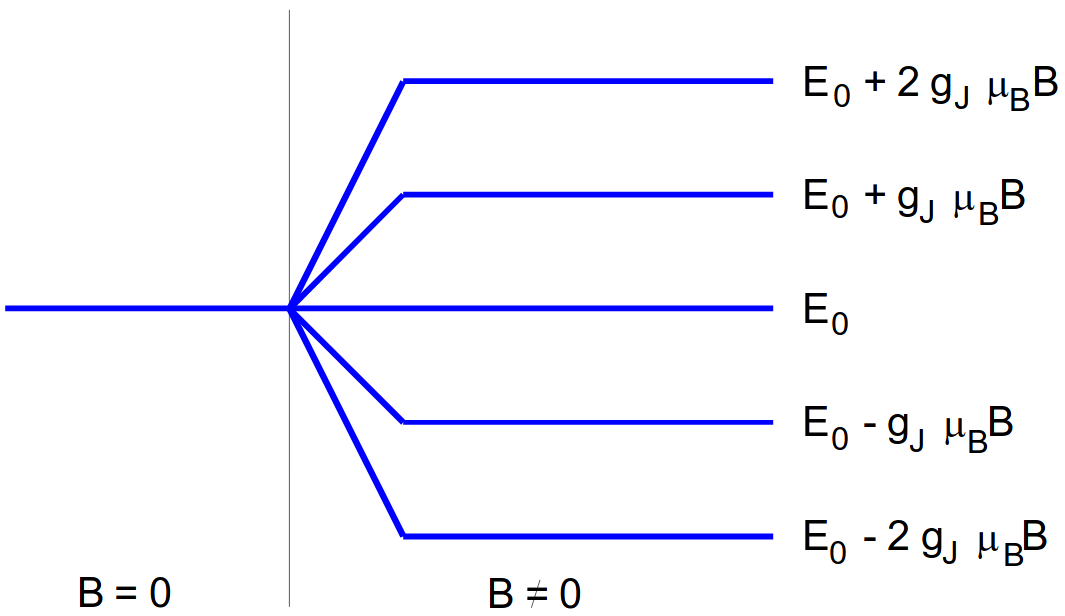
\includegraphics[width=.5\textwidth]{ressources/Aufspaltung.png}
  \caption{Aufspaltung der Energieniveaus ($J=2$), verursacht durch ein B-Feld\cite{skript}.}
  \label{fig:theorie_1}
\end{figure}

\subsection{Auswahlregeln}
Um eine Aussage über mögliche Übergänge der neuen Niveaus treffen zu können, werden sogenannte Auswahlregeln benötigt. Ausgangspunkt ist dabei die zeitabhängige Schrödingergleichung. Diese wird gelöst und normiert. Mit der Erkenntnis, dass die Dichteverteilung eine zeitabhängige Größe ist, mit der mathematischen Beschreibung des gesamten Dipolmoments und mit der Wellenfunktion des Atoms folgen schließlich die Auswahlregeln:
\begin{align}
	\Delta m=0 \quad \text{und} \quad \Delta m=\pm1
\end{align}

Die Auswahlregeln erzeugen dabei verschiedene Eigenschaften im Bereich der imitierten Strahlung aufweisen. Aufgrund der Winkelabhängigkeit der Strahlungsintensität, schwingt der Dipol mit der Auswahlregel $\Delta m=0$ zwar parallel zum angelegten B-Feld, strahlt aber nicht in dieser Richtung ab. Somit ergibt sich die maximale Intensität senkrecht zur Feldrichtung. Zusammenfassend ergibt sich also eine linear polarisierte Welle parallel zum B-Feld. In dem Fall $\Delta m=-1$ erzeugt der Dipol einer zirkularpolarisierte Schwingung um die Feldausrichtung des B-Feld. Bei $\Delta m=+1$ entsteht ebenfalls eine zirkularpolarisierte Schwingung, jedoch in entgegengesetzter Richtung

\subsection{normaler Zeeman-Effekt}
Beim normalen Zeeman-Effekt bezieht man sich auf den Fall $S=0$. Alle zuvor getroffen Aussagen, besonders über die Energiedifferenz und die Auswahlregeln, gelten weiterhin. Die getroffene Einschränkung bewirkt lediglich, dass die für jedes $J$ gilt:
\begin{align}
	g_J=1 \qquad \text{und} \qquad \Delta E_{mag}=m\mu_B B
\end{align}
Dies hat zur Folge, dass der Abstand zwischen allen Niveaus äquidistant ist. In Abbildung \ref{fig:theorie_2} ist ein Beispiel für den normalen Zeeman-Effekt dargestellt.


\begin{figure}[H]
  \centering
  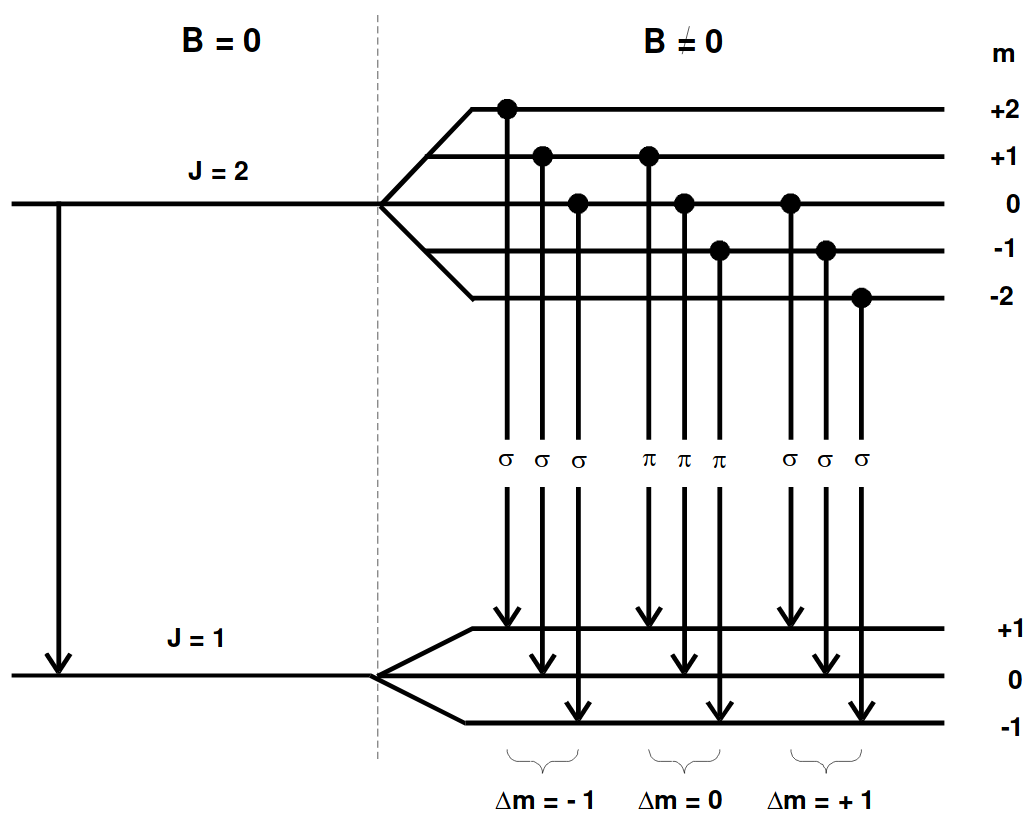
\includegraphics[width=.5\textwidth]{ressources/anomal.png}
  \caption{Aufspaltung der Energieniveaus und Polarisation der Spektrallinien beim normalen Zeeman-Effekt\cite{skript}.}
  \label{fig:theorie_2}
\end{figure}

Aufgrund der drei Auswahlregeln, sind die Übergänge in drei Gruppen aufzuteilen. In einer Gruppe erfüllen die Übergänge die gleiche Auswahlregel. Wegen der unterschiedlichen Polarisation, bedingt durch die Auswahlregel, sind nicht alle Linien an jedem Beobachtungspunkt sichtbar. Bei $\Delta m=0$ bleibt die Energie konstant beim Übergang. Dieser Fall wird als $\pi$-Komponente bezeichnet und erzeugt eine lineare polarisierte Spektrallinie in Feldrichtung. Diese ist nur bei Beobachtung senkrecht zu Feldausrichtung möglich, da dann die Intensität maximal wird. Somit ist sie longitudinal nicht zu beobachten. Im Fall $\Delta m=\pm1$ sind die Energien um $E=\mu_B B$ verschoben. Die Spektrallinien sind zirkularpolarisiert um die Feldrichtung und erscheinen in transversale Beobachtungsrichtung linearpolarisiert. Somit sind die als $\sigma_\pm$-Komponente bezeichneten Spektrallinien in jeder Beobachtungsrichtung sichtbar. Zur Verdeutlichung ist in Abbildung \ref{fig:theorie_3} das Aufspaltungsbild sowohl longitudinal als auch transversal dargestellt.

\begin{figure}[H]
  \centering
  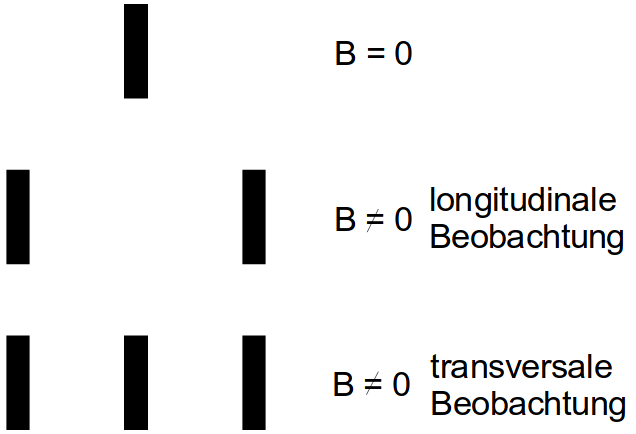
\includegraphics[width=.45\textwidth]{ressources/Beobachtungspunkt.png}
  \caption{Intensität der emittierten Strahlung aus longitudinaler und transversaler Sicht\cite{skript}.}
  \label{fig:theorie_3}
\end{figure}


\subsection{anomaler Zeeman-Effekt}
Dieser tritt weitaus häufiger auf als der normale Zeeman-Effekt, da für diesen die Spinkomponente ungleich Null ist. Durch die Quantenmechanik kann erneut gezeigt werden, dass sich die Auswahlregel nicht ändern. Der größte Unterschied besteht lediglich darin, dass die Energieunterschiede zwischen den Übergänge nicht mehr äquidistant sind. Grund dafür ist der Land\'{e}-Faktor der zu einem linienreicheren Spektrum führt.



%     \centering
%     \begin{subfigure}[b]{0.475\textwidth}
%         \centering
%         \includegraphics[width=\textwidth]{Abbildungen/Schaltung1.pdf}
%         \caption[]%
%         {{\small Schaltung 1.}}
%         \label{fig:Schaltung1}
%     \end{subfigure}
%     \hfill
%     \begin{subfigure}[b]{0.475\textwidth}
%         \centering
%         \includegraphics[width=\textwidth]{Abbildungen/Schaltung2.pdf}
%         \caption[]%
%         {{\small Schaltung 2.}}
%         \label{fig:Schaltung2}
%     \end{subfigure}
%     \vskip\baselineskip
%     \begin{subfigure}[b]{0.475\textwidth}
%         \centering
%         \includegraphics[width=\textwidth]{Abbildungen/Schaltung4.pdf}    % Zahlen vertauscht ... -.-
%         \caption[]%
%         {{\small Schaltung 3.}}
%         \label{fig:Schaltung3}
%     \end{subfigure}
%     \quad
%     \begin{subfigure}[b]{0.475\textwidth}
%         \centering
%         \includegraphics[width=\textwidth]{Abbildungen/Schaltung3.pdf}
%         \caption[]%
%         {{\small Schaltung 4.}}
%         \label{fig:Schaltung4}
%     \end{subfigure}
%     \caption[]
%     {Ersatzschaltbilder der verschiedenen Teilaufgaben.}
%     \label{fig:Schaltungen}
% \end{figure*}
